\section*{练习题}
\begin{enumerate}
\item 
\begin{question}
构建图\ref{exerc:exercise1-4}和图\ref{exerc:exercise1-2}  所示物体的三维模型。
\begin{figure}[htbp]
\centering
\begin{floatrow}[2]
\ffigbox{\caption{ }\label{exerc:exercise1-4}}{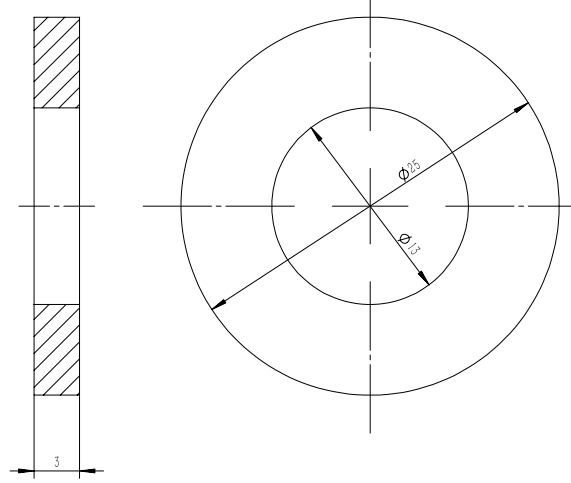
\includegraphics[scale=0.35]{exercise1-4}}
\ffigbox{\caption{ }\label{exerc:exercise1-2}}{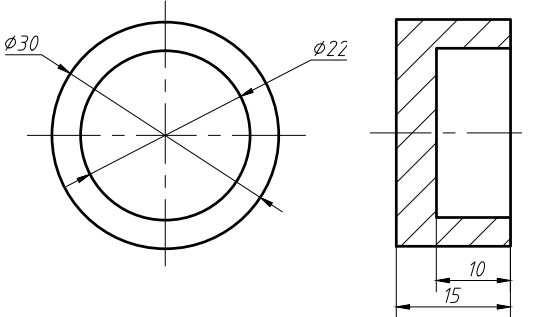
\includegraphics[scale=0.5]{exercise1-2}}
\end{floatrow}
\end{figure}
\end{question}

\item 
\begin{question}
构建图\ref{exerc:exercise1-3}和图\ref{exerc:exercise1-1}  所示物体的三维模型。
\begin{figure}[htbp]
\centering
\begin{floatrow}[2]
\ffigbox{\caption{ }\label{exerc:exercise1-3}}{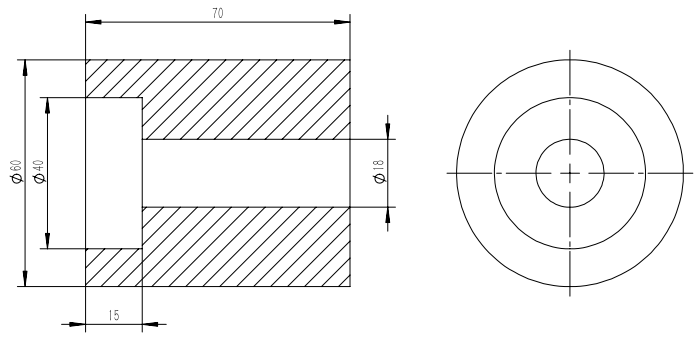
\includegraphics[scale=0.45]{exercise1-3}}
\ffigbox{\caption{ }\label{exerc:exercise1-1}}{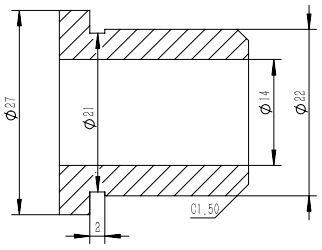
\includegraphics[scale=0.6]{exercise1-1}}
\end{floatrow}
\end{figure}
\end{question}

\item 
\begin{question}
构建图\ref{exerc:exercise1-5} 所示物体的三维模型。
\begin{figure}[htbp]
\centering
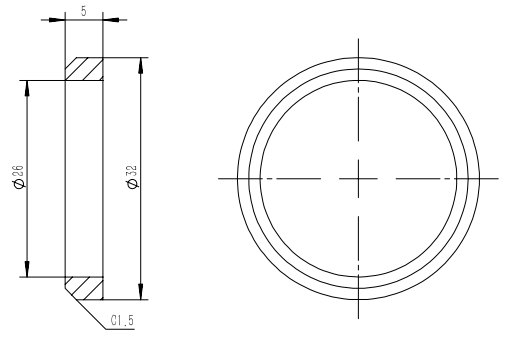
\includegraphics[scale=0.6]{exercise1-5}
\caption{ }\label{exerc:exercise1-5}
\end{figure}
\end{question}
\end{enumerate}
\endinput